
\chapter{对抗学习}
\thispagestyle{empty}

\setlength{\fboxrule}{0pt}\setlength{\fboxsep}{0cm}
\noindent\shadowbox{
\begin{tcolorbox}[arc=0mm,colback=lightblue,colframe=darkblue,title=学习目标与要求]
%\kai\textcolor{darkblue}{1.~~GAN学习.} \\ 

\end{tcolorbox}}
\setlength{\fboxrule}{1pt}\setlength{\fboxsep}{4pt} 


\section{GAN的技术应用} 

在我们实际大数据环境中,我们需要从数据中挖掘出基本的结构化信息,
从而可以帮助我们有效构造样本,解决一些传统监督学习所无法解决的
问题;比方说,正样本覆盖率低,负样本缺失,模型overfitting,
鲁棒性不够等等;生成式模型的目的是找到一个函数可以最大的似然数据
的真实分布;通常我们用 $f(X:\theta$ 来表示这样的一个函数,
找到一个使生成的数据最像真实数据的过程就是一个MLE的过程。
问题是:当数据的分布比较复杂时,简单的函数无法表达样本空间;
现在通过深度网络结构可以表达一个更加复杂的函数,但是训练过程
成为了关键。基于sampling的训练过程显示不是高效的;早年
graphical model会采用变分推断方法;还有今年出现的对抗学习
方法;GAN相关技术的演变如下图所示:


\begin{figure}[h]
\centering
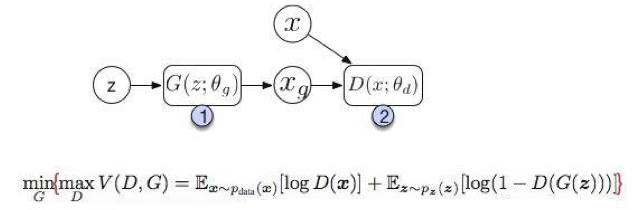
\includegraphics[totalheight=1.8in]{fig/standard_gan.png}
\caption{ 标准GAN算法示意图 } \label{fig:gansamples}
\end{figure}

最经典的GAN模型,由Ian Goodfellow提出,先从一个简单的分布中
采样一个噪声信号,然后经过生成函数后映射到我们想去拟合的数据分布
$x_g$。生成的数据和真实数据都会输入到一个识别网络D,识别网络
通过判别输出一个标量,表示数据来自真实数据的概率。在实现上,
要求G和D都是可微分函数,可以用多层神经网络来实现;后半部分是
模型训练中的目标函数。从公式上看,类似于CrossEntropy,注意到
D是P(Xdata)的近似。对于D来说,要尽量使公式最大化(识别能力强), 
而对于G又想使其最小。整个训练过程是一个迭代过程,但是在迭代中,
对D的优化又是内循环。生成模型可以发挥价值的场所: 
\begin{description}
	\item 特征表示
	\item 强化学习中的探索
	\item 逆强化学习
	\item 迁移学习
\end{description}

\section{深度学习中的Lipschitz约束:泛化与生成模型} 
记输入为 x,输出为 y,模型为 f,模型参数为 w,记为:$$y=f_w(x)$$ 我们希望得到一个稳健的模型,一个模型的稳健体现在两个方面;1). 对于参数扰动的稳定;2). 对于输入扰动的稳定; 这里先阐述一个L-约束的概念,就是希望当,$$ x_1-x_2 $$, 值 $$||f_w(x_1)-f_w(x_2)||$$ 也尽可能小;利普希孜约束是一种具体的表达形式;$$ ||f_w(x_1)-f_w(x_2)|| \leq C(w) \times || x_1-x_2 || $$; 也就是说,希望整个模型被一个线性函数控制住;这里面需要再给大家介绍一个普范数的概念,这个会被应用在WGAN算法中,来实现判别器模型的稳定;

images/gan/20210715150331.png

这里再介绍另外一个用来度量两个分布的最有传输理论,对于生成模型,运用optimal transport理论来实现判别器对于度量真实数据在参数空间下的分布与生成数据在参数空间下的分布差异化的精细化度量,从而来给与生成器更加有效的指引;从而一定程度的解决GAN训练稳定性和模式坍塌问题;在原始GAN算法中,判别器一般通过JS divergence来优化,但是JS divergence有致命的缺陷,就是两个分布互不相交的情况下,两个分布的JS divergence永远都是常熟log2,并且由于generator生成的分布和真实数据分布的支撑集都是高维空间下的低维流形,所以他们重叠的部分测度几乎为0,这样无法度量两个分布在不相交情况下的距离,计算梯度的时候会出现0-grandient现象;因此我们采用optimal transport distance来解决这个问题,但是随着随机变量表征维度的增长,问题的规模是成指数增加的,对于一张32*32的图片,我们面对的输入的随机变量的维度是1000,因此问题的规模是2^1000, 这是很难计算的;下面我们需要思考来解这个问题,最有传输问题本质是一个线性规划问题,我们需要优化的问题以及约束条件都是线性的函数;因此我可以考虑通过对偶问题来求:并且对偶问题的解是原问题的下届;

$$
	OT(p||Q) = sup_{f\in L} ( \int \phi(x) P(x)dx + \int \psi(y)Q(y)dy ) 
$$
其中,$$L= \{ f | \psi(y)+\phi(x)\leq c(x,y) \}$$
直观的解释这个公式,L中的某个f,该f在不同分布P,Q下的期望之差最大;

GAN 模型的评估手段,目前用来衡量不同GAN模型的实验指标都存在很大的问题,通常我们会用一个分类器来看看我们对于生成的instance分类的准确率来评估;但是任何一个分类器都很难覆盖所有可能的图片类别,因此他的分类精度就不是完美的;

什么是模式坍塌,具体来说就是,给定一个Z,当z发生变化时,G(Z)没有发生变化,那么在这个局部,GAN就发生了模式坍塌,也就是说不能产生连续变化的样本;这个现象从几何角度思考的话,就是对应的流型在这个局部点,沿着不同的且向量方向不再变化;换言之,所有切向量不再彼此相互独立--某些切向量要么消失,要么相互之间变得相互依赖,导致流型的维度在局部出现缺陷;

1. 比较理论的研究可以专注于,有了这些局部参数表示,如何去定义出一整套黎曼流型的数学结构,比如局部的曲率,黎曼度量,和如果沿着流型去算测地线和两个数据点之间的测地距离。

2. 从应用的角度,给定了一个图像x,用局部表示G(x,z)可以对这个x在它的局部领域中做各种编辑操作或者控制图像的各种属性。这个可以结合有监督的对局部参数的意义进行训练。



\begin{thebibliography}{99}
\addcontentsline{toc}{chapter}{\protect\numberline{}{\hspace{-1.5em}参考文献}}
\markboth{参考文献}{参考文献}
\bibitem{1} Gan导读,http://weibo.com/ttarticle/p/show?id=2309404060390806926698
\bibitem{2} John Glover, Modeling documents with generative adversarial networks, workshop on adversarial training, NIPS 2016, Barcelona, Spain

\end{thebibliography}

 
